%%%%%%%%%%%%%%%%%%%%%%%%%%%%%%%%%%%%%%%%%%%%%%%%%%%%%%%%%%%%%%%%%%
%%%%%%%%%%%%%%%%%%%%%%%%%%%%%%%%%%%%%%%%%%%%%%%%%%%%%%%%%%%%%%%%%%
% \setmathfont{TeX Gyre Termes Math}
%Packages
\documentclass[10pt, a4paper]{article}
\usepackage[top=3cm, bottom=4cm, left=2cm, right=2cm]{geometry}
\usepackage{amsmath,amsthm,amsfonts,amssymb,amscd, fancyhdr, color, comment, graphicx, environ}
\usepackage{float}
\usepackage{booktabs}
\usepackage{pifont}
\usepackage{mathrsfs}
\usepackage[math-style=ISO]{unicode-math}
\usepackage{lastpage}
\usepackage[dvipsnames]{xcolor}
\usepackage[framemethod=TikZ]{mdframed}
\usepackage{enumerate}
\usepackage[shortlabels]{enumitem}
\usepackage{fancyhdr}
\usepackage{indentfirst}
\usepackage{listings}
\usepackage{sectsty}
\usepackage{thmtools}
\usepackage{shadethm}
\usepackage{hyperref}
\usepackage{setspace}
\usepackage{adjustbox}
\hypersetup{
	colorlinks=true,
	linkcolor=blue,
	filecolor=magenta,
	urlcolor=blue,
}
\usepackage{xcolor,colortbl}
%%%%%%%%%%%%%%%%%%%%%%%%%%%%%%%%%%%%%%%%%%%%%%%%%%%%%%%%%%%%%%%%%%
%%%%%%%%%%%%%%%%%%%%%%%%%%%%%%%%%%%%%%%%%%%%%%%%%%%%%%%%%%%%%%%%%%
%Environment setup
\mdfsetup{skipabove=\topskip,skipbelow=\topskip}
\newrobustcmd\ExampleText{%
	An \textit{inhomogeneous linear} differential equation has the form
	\begin{align}
		L[v ] = f,
	\end{align}
	where $L$ is a linear differential operator, $v$ is the dependent
	variable, and $f$ is a given non−zero function of the independent
	variables alone.
}
\mdfdefinestyle{theoremstyle}{%
	linecolor=black,linewidth=1pt,%
	frametitlerule=true,%
	frametitlebackgroundcolor=gray!20,
	innertopmargin=\topskip,
}
\mdtheorem[style=theoremstyle]{Problem}{Question Number}
\setcounter{Problem}{2}
\newenvironment{Solution}{\textbf{Solution.}}

\definecolor{codegreen}{rgb}{0,0.6,0}
\definecolor{codegray}{rgb}{0.5,0.5,0.5}
\definecolor{codepurple}{rgb}{0.58,0,0.82}
\definecolor{backcolour}{rgb}{0.95,0.95,0.92}

\lstdefinestyle{mystyle}{
	backgroundcolor=\color{backcolour},
	commentstyle=\color{codegreen},
	keywordstyle=\color{magenta},
	numberstyle=\tiny\color{codegray},
	stringstyle=\color{codepurple},
	basicstyle=\ttfamily\footnotesize,
	breakatwhitespace=false,
	breaklines=true,
	captionpos=b,
	keepspaces=true,
	numbers=left,
	numbersep=5pt,
	showspaces=false,
	showstringspaces=false,
	showtabs=false,
	tabsize=2
}

\lstset{style=mystyle}
%%%%%%%%%%%%%%%%%%%%%%%%%%%%%%%%%%%%%%%%%%%%%%%%%%%%%%%%%%%%%%%%%%
%%%%%%%%%%%%%%%%%%%%%%%%%%%%%%%%%%%%%%%%%%%%%%%%%%%%%%%%%%%%%%%%%%
%Fill in the appropriate information below
\newcommand{\norm}[1]{\left\lVert#1\right\rVert}
\newcommand\course{XXXX0000}                            % <-- course name   
\newcommand\hwnumber{0}                                 % <-- homework number
\newcommand\Information{Someone}                        % <-- personal information
%%%%%%%%%%%%%%%%%%%%%%%%%%%%%%%%%%%%%%%%%%%%%%%%%%%%%%%%%%%%%%%%%%
%%%%%%%%%%%%%%%%%%%%%%%%%%%%%%%%%%%%%%%%%%%%%%%%%%%%%%%%%%%%%%%%%%
%Page setup
\pagestyle{fancy}
\headheight 35pt
\lhead{\today \hspace*{4cm} Key-Breakers}
\rhead{
\includegraphics[width=1.2cm]{../logo.png}}
\lfoot{}
\pagenumbering{arabic}
\cfoot{\small\thepage}
\rfoot{}
\headsep 1.2em
\renewcommand{\baselinestretch}{1.25}
%%%%%%%%%%%%%%%%%%%%%%%%%%%%%%%%%%%%%%%%%%%%%%%%%%%%%%%%%%%%%%%%%%
%%%%%%%%%%%%%%%%%%%%%%%%%%%%%%%%%%%%%%%%%%%%%%%%%%%%%%%%%%%%%%%%%%
%Add new commands here
\renewcommand{\labelenumi}{\alph{enumi})}
\newcommand{\Z}{\mathbb Z}
\newcommand{\R}{\mathbb R}
\newcommand{\Q}{\mathbb Q}
\newcommand{\NN}{\mathbb N}
\newcommand{\PP}{\mathbb P}
\DeclareMathOperator{\Mod}{Mod}
\renewcommand\lstlistingname{Algorithm}
\renewcommand\lstlistlistingname{Algorithms}
\def\lstlistingautorefname{Alg.}
\newtheorem*{theorem}{Theorem}
\newtheorem*{lemma}{Lemma}
\newtheorem{case}{Case}
\newcommand{\assign}{:=}
\newcommand{\infixiff}{\text{ iff }}
\newcommand{\nobracket}{}
\newcommand{\backassign}{=:}
\newcommand{\tmmathbf}[1]{\ensuremath{\boldsymbol{#1}}}
\newcommand{\tmop}[1]{\ensuremath{\operatorname{#1}}}
\newcommand{\tmtextbf}[1]{\text{{\bfseries{#1}}}}
\newcommand{\tmtextit}[1]{\text{{\itshape{#1}}}}

\newenvironment{itemizedot}{
	\begin{itemize}
		\renewcommand{\labelitemi}{$\bullet$}
		\renewcommand{\labelitemii}{$\bullet$}
		\renewcommand{\labelitemiii}{$\bullet$}
		\renewcommand{\labelitemiv}{$\bullet$}}
		{\end{itemize}}

\catcode`\<=\active\def<{
\fontencoding{T1}\selectfont\symbol{60}\fontencoding{\encodingdefault}}
\catcode`\>=\active\def>{
\fontencoding{T1}\selectfont\symbol{62}\fontencoding{\encodingdefault}}
\catcode`\<=\active\def<{
\fontencoding{T1}\selectfont\symbol{60}\fontencoding{\encodingdefault}}

%%%%%%%%%%%%%%%%%%%%%%%%%%%%%%%%%%%%%%%%%%%%%%%%%%%%%%%%%%%%%%%%%%
%%%%%%%%%%%%%%%%%%%%%%%%%%%%%%%%%%%%%%%%%%%%%%%%%%%%%%%%%%%%%%%%%%
%Begin now!



\begin{document}
%%%%%%%%%%%%%%%%%%%%%%%%%%%%%%%%%%%%%%%%%%%%%%%%%%%%%%%%%%%%%%%%%%
%%%%%%%%%%%%%%%%%%%%%%%%%%%%%%%%%%%%%%%%%%%%%%%%%%%%%%%%%%%%%%%%%%
%Start the assignment now
%%%%%%%%%%%%%%%%%%%%%%%%%%%%%%%%%%%%%%%%%%%%%%%%%%%%%%%%%%%%%%%%%%
%New problem
\newpage
\begin{Problem}
	\begin{itemize}
		\item Using your favorite programming language implement the AES key-expansion algorithm
		\item Now use the state matrix initialized with your name in Problem 1 as your initial key
		\item Show the 10 rounds keys in the main assignment1.
		\item For the fifth round-key show all the steps of the key-expansion algorithm that leads to
		      the sixth round key.
	\end{itemize}
\end{Problem}

\begin{Solution}
	\begin{itemize}
		\item \textbf{AES Key Expansion Algorithm}
		      \begin{center}
			      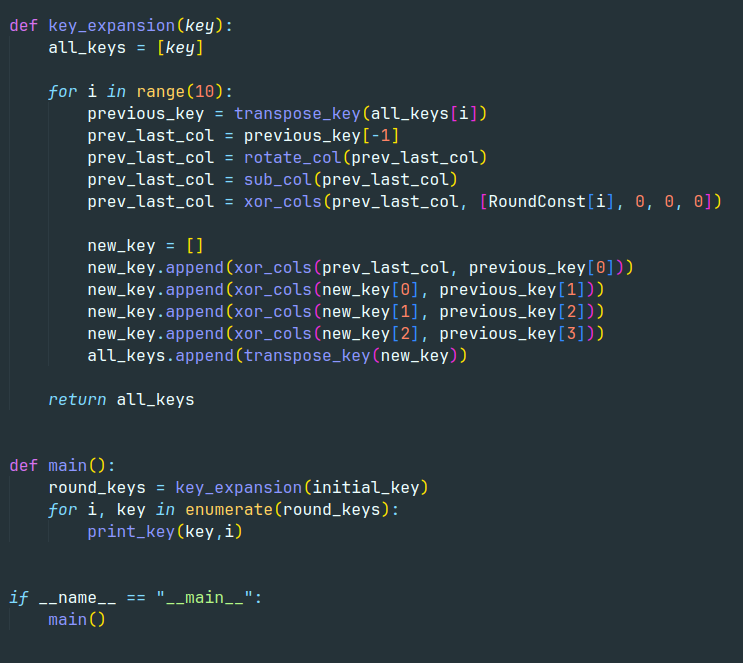
\includegraphics[width=15cm]{p1.png}
		      \end{center}

		      \pagebreak
		\item \textbf{Initial Key}
		      \textbf{Note}

		      \begin{itemize}
			      \item [1. ]
			            Dump initial key. The initial key taken from python code in file with name \texttt{Key\_Expansion.py}
			            (when python code rerun this key will be updated)
			      \item [2. ]

			            Python File \texttt{Key\_Expansion.py} should \textbf{run in the directory \texttt{Question\_03}}(As it is creating
			            \texttt{.tex} file in current directory, which is then used by the latex code to fetch keys)
		      \end{itemize}

		      \[
    \text{Initial Key : }
    \renewcommand{\arraystretch}{1.5}
    \setlength{\arrayrulewidth}{0.6mm}
    \setlength{\tabcolsep}{0.5em}
    \begin{array}{|>{\centering\arraybackslash}m{2em}|>{\centering\arraybackslash}m{2em}|>{\centering\arraybackslash}m{2em}|>{\centering\arraybackslash}m{2em}|}
        \hline
        \text{0xB3} & \text{0x2F} & \text{0x2F} & \text{0x63} \\
        \hline
        \text{0xB7} & \text{0x3B} & \text{0x63} & \text{0x83} \\
        \hline
        \text{0x29} & \text{0x63} & \text{0x00} & \text{0xED} \\
        \hline
        \text{0x63} & \text{0x83} & \text{0xFC} & \text{0xB7} \\
        \hline
    \end{array}
\]


		\item \textbf{All 10 Round Keys}

		      \begin{itemize}
			      \item [1. ]
			            Dump all round keys.All round keys taken from output of python code in
			            file with name \texttt{Key\_Expansion.py} (when python code rerun these keys will be updated)
			      \item [2. ]

			            Python File \texttt{Key\_Expansion.py} should \textbf{run in the directory \texttt{Question\_03}}(As it is creating
			            \texttt{.tex} file in current directory, which is then used by the latex code to fetch all round keys)
			      \item [3. ]
			            All Round keys are shown on \textbf{next page}.
		      \end{itemize}
		      \pagebreak
		      \[
    \renewcommand{\arraystretch}{1.5}
    \setlength{\arrayrulewidth}{0.6mm}
    \setlength{\tabcolsep}{0.5em}
    \begin{tabular}{c c}
        \text{Round 1 Key : }
        \begin{array}{|>{\centering\arraybackslash}m{2em}|>{\centering\arraybackslash}m{2em}|>{\centering\arraybackslash}m{2em}|>{\centering\arraybackslash}m{2em}|}
            \hline
            \text{0x5E} & \text{0x71} & \text{0x5E} & \text{0x3D} \\
            \hline
            \text{0xE2} & \text{0xD9} & \text{0xBA} & \text{0x39} \\
            \hline
            \text{0x80} & \text{0xE3} & \text{0xE3} & \text{0x0E} \\
            \hline
            \text{0x98} & \text{0x1B} & \text{0xE7} & \text{0x50} \\
            \hline
        \end{array}
        &
        \text{Round 2 Key : }
        \begin{array}{|>{\centering\arraybackslash}m{2em}|>{\centering\arraybackslash}m{2em}|>{\centering\arraybackslash}m{2em}|>{\centering\arraybackslash}m{2em}|}
            \hline
            \text{0x4E} & \text{0x3F} & \text{0x61} & \text{0x5C} \\
            \hline
            \text{0x49} & \text{0x90} & \text{0x2A} & \text{0x13} \\
            \hline
            \text{0xD3} & \text{0x30} & \text{0xD3} & \text{0xDD} \\
            \hline
            \text{0xBF} & \text{0xA4} & \text{0x43} & \text{0x13} \\
            \hline
        \end{array}
        \\
        \vspace{1em} \\ 
        \text{Round 3 Key : }
        \begin{array}{|>{\centering\arraybackslash}m{2em}|>{\centering\arraybackslash}m{2em}|>{\centering\arraybackslash}m{2em}|>{\centering\arraybackslash}m{2em}|}
            \hline
            \text{0x37} & \text{0x08} & \text{0x69} & \text{0x35} \\
            \hline
            \text{0x88} & \text{0x18} & \text{0x32} & \text{0x21} \\
            \hline
            \text{0xAE} & \text{0x9E} & \text{0x4D} & \text{0x90} \\
            \hline
            \text{0xF5} & \text{0x51} & \text{0x12} & \text{0x01} \\
            \hline
        \end{array}
        &
        \text{Round 4 Key : }
        \begin{array}{|>{\centering\arraybackslash}m{2em}|>{\centering\arraybackslash}m{2em}|>{\centering\arraybackslash}m{2em}|>{\centering\arraybackslash}m{2em}|}
            \hline
            \text{0xC2} & \text{0xCA} & \text{0xA3} & \text{0x96} \\
            \hline
            \text{0xE8} & \text{0xF0} & \text{0xC2} & \text{0xE3} \\
            \hline
            \text{0xD2} & \text{0x4C} & \text{0x01} & \text{0x91} \\
            \hline
            \text{0x63} & \text{0x32} & \text{0x20} & \text{0x21} \\
            \hline
        \end{array}
        \\
        \vspace{1em} \\ 
        \text{Round 5 Key : }
        \begin{array}{|>{\centering\arraybackslash}m{2em}|>{\centering\arraybackslash}m{2em}|>{\centering\arraybackslash}m{2em}|>{\centering\arraybackslash}m{2em}|}
            \hline
            \text{0xC3} & \text{0x09} & \text{0xAA} & \text{0x3C} \\
            \hline
            \text{0x69} & \text{0x99} & \text{0x5B} & \text{0xB8} \\
            \hline
            \text{0x2F} & \text{0x63} & \text{0x62} & \text{0xF3} \\
            \hline
            \text{0xF3} & \text{0xC1} & \text{0xE1} & \text{0xC0} \\
            \hline
        \end{array}
        &
        \text{Round 6 Key : }
        \begin{array}{|>{\centering\arraybackslash}m{2em}|>{\centering\arraybackslash}m{2em}|>{\centering\arraybackslash}m{2em}|>{\centering\arraybackslash}m{2em}|}
            \hline
            \text{0x8F} & \text{0x86} & \text{0x2C} & \text{0x10} \\
            \hline
            \text{0x64} & \text{0xFD} & \text{0xA6} & \text{0x1E} \\
            \hline
            \text{0x95} & \text{0xF6} & \text{0x94} & \text{0x67} \\
            \hline
            \text{0x18} & \text{0xD9} & \text{0x38} & \text{0xF8} \\
            \hline
        \end{array}
        \\
        \vspace{1em} \\ 
        \text{Round 7 Key : }
        \begin{array}{|>{\centering\arraybackslash}m{2em}|>{\centering\arraybackslash}m{2em}|>{\centering\arraybackslash}m{2em}|>{\centering\arraybackslash}m{2em}|}
            \hline
            \text{0xBD} & \text{0x3B} & \text{0x17} & \text{0x07} \\
            \hline
            \text{0xE1} & \text{0x1C} & \text{0xBA} & \text{0xA4} \\
            \hline
            \text{0xD4} & \text{0x22} & \text{0xB6} & \text{0xD1} \\
            \hline
            \text{0xD2} & \text{0x0B} & \text{0x33} & \text{0xCB} \\
            \hline
        \end{array}
        &
        \text{Round 8 Key : }
        \begin{array}{|>{\centering\arraybackslash}m{2em}|>{\centering\arraybackslash}m{2em}|>{\centering\arraybackslash}m{2em}|>{\centering\arraybackslash}m{2em}|}
            \hline
            \text{0x74} & \text{0x4F} & \text{0x58} & \text{0x5F} \\
            \hline
            \text{0xDF} & \text{0xC3} & \text{0x79} & \text{0xDD} \\
            \hline
            \text{0xCB} & \text{0xE9} & \text{0x5F} & \text{0x8E} \\
            \hline
            \text{0x17} & \text{0x1C} & \text{0x2F} & \text{0xE4} \\
            \hline
        \end{array}
        \\
        \vspace{1em} \\ 
        \text{Round 9 Key : }
        \begin{array}{|>{\centering\arraybackslash}m{2em}|>{\centering\arraybackslash}m{2em}|>{\centering\arraybackslash}m{2em}|>{\centering\arraybackslash}m{2em}|}
            \hline
            \text{0xAE} & \text{0xE1} & \text{0xB9} & \text{0xE6} \\
            \hline
            \text{0xC6} & \text{0x05} & \text{0x7C} & \text{0xA1} \\
            \hline
            \text{0xA2} & \text{0x4B} & \text{0x14} & \text{0x9A} \\
            \hline
            \text{0xD8} & \text{0xC4} & \text{0xEB} & \text{0x0F} \\
            \hline
        \end{array}
        &
        \text{Round 10 Key : }
        \begin{array}{|>{\centering\arraybackslash}m{2em}|>{\centering\arraybackslash}m{2em}|>{\centering\arraybackslash}m{2em}|>{\centering\arraybackslash}m{2em}|}
            \hline
            \text{0xAA} & \text{0x4B} & \text{0xF2} & \text{0x14} \\
            \hline
            \text{0x7E} & \text{0x7B} & \text{0x07} & \text{0xA6} \\
            \hline
            \text{0xD4} & \text{0x9F} & \text{0x8B} & \text{0x11} \\
            \hline
            \text{0x56} & \text{0x92} & \text{0x79} & \text{0x76} \\
            \hline
        \end{array}
        \\
        \vspace{1em} \\ 
    \end{tabular}
\]


		\item \textbf{AES Key Expansion - Stepwise Solution for Round 5 Key}

		      Below is a stepwise explanation of the transformations involved in generating the round key for the sixth round, from the fifth round key

		      \textbf{Note : Following result is generated from the python code}


		      \begin{enumerate}[label=\textbf{Step \arabic*:}]
			      \item \textbf{Initial Fifth Round Key}

The initial key is provided as a 4x4 matrix at the start of the fifth round:

\[
    \text{Fifth Round Key : }
    \renewcommand{\arraystretch}{1.5}
    \setlength{\arrayrulewidth}{0.6mm}
    \setlength{\tabcolsep}{0.5em}
    \begin{array}{|>{\centering\arraybackslash}m{2em}|>{\centering\arraybackslash}m{2em}|>{\centering\arraybackslash}m{2em}|>{\centering\arraybackslash}m{2em}|}
        \hline
        \text{0xC3} & \text{0x09} & \text{0xAA} & \text{0x3C} \\
        \hline
        \text{0x69} & \text{0x99} & \text{0x5B} & \text{0xB8} \\
        \hline
        \text{0x2F} & \text{0x63} & \text{0x62} & \text{0xF3} \\
        \hline
        \text{0xF3} & \text{0xC1} & \text{0xE1} & \text{0xC0} \\
        \hline
    \end{array}
\]

\item \textbf{Rotate the Last Column}

The last column is rotated as follows:
\[
    \begin{array}{c@{\hskip 2cm}c}
        \text{Last Column Before Rotation} & \text{Last Column After Rotation} \\[1em]
        \begin{array}{|c|}\n            \hline\n\text{0x3C}            \\ \hline
\text{0xB8}            \\ \hline
\text{0xF3}            \\ \hline
\text{0xC0} \\ \hline\n        \end{array}\n        &
        \begin{array}{|c|}\n            \hline\n\text{0xB8}            \\ \hline
\text{0xF3}            \\ \hline
\text{0xC0}            \\ \hline
\text{0x3C} \\ \hline\n        \end{array}\n    \end{array}\n\]

\item \textbf{Substitute Bytes}

Apply the S-Box substitution to the rotated column:
\[
    \begin{array}{c@{\hskip 2cm}c}
        \text{Last Column Before Substitution} & \text{Last Column After Substitution} \\[1em]
        \begin{array}{|c|}\n            \hline\n\text{0xB8}            \\ \hline
\text{0xF3}            \\ \hline
\text{0xC0}            \\ \hline
\text{0x3C} \\ \hline\n        \end{array}\n        &
        \begin{array}{|c|}\n            \hline\n\text{0x6C}            \\ \hline
\text{0x0D}            \\ \hline
\text{0xBA}            \\ \hline
\text{0xEB} \\ \hline\n        \end{array}\n    \end{array}\n\]
\pagebreak
\item \textbf{Apply Round Constant}

XOR the substituted column with the round constant.

\[
\begin{align*}
    & 
    \begin{array}{|c|}\hline\n\text{0x6C} \\ \hline\n\text{0x0D} \\ \hline\n\text{0xBA} \\ \hline\n\text{0xEB} \\ \hline\n\end{array} 
    \quad \oplus \quad
    \begin{array}{|c|}\hline\n\text{0x20} \\ \hline\n\text{0x00} \\ \hline\n\text{0x00} \\ \hline\n\text{0x00} \\ \hline\n\end{array} 
    \quad = \quad
    \begin{array}{|c|}\hline\n\text{0x4C} \\ \hline\n\text{0x0D} \\ \hline\n\text{0xBA} \\ \hline\n\text{0xEB} \\ \hline\n\end{array}
\end{align*}
\]\item \textbf{Generating the next round key }

The new key word is generated by XORing the resulting column with the previous column.
\[
        \begin{align*}
            & 
            \begin{array}{|c|}\hline\n\text{0xC3} \\ \hline\n\text{0x69} \\ \hline\n\text{0x2F} \\ \hline\n\text{0xF3} \\ \hline\n\end{array} 
            \quad \oplus \quad
            \begin{array}{|c|}\hline\n\text{0x4C} \\ \hline\n\text{0x0D} \\ \hline\n\text{0xBA} \\ \hline\n\text{0xEB} \\ \hline\n\end{array} 
            \quad = \quad
            \begin{array}{|c|}\hline\n\text{0x8F} \\ \hline\n\text{0x64} \\ \hline\n\text{0x95} \\ \hline\n\text{0x18} \\ \hline\n\end{array}
        \end{align*}
        \]\[
        \begin{align*}
            & 
            \begin{array}{|c|}\hline\n\text{0x09} \\ \hline\n\text{0x99} \\ \hline\n\text{0x63} \\ \hline\n\text{0xC1} \\ \hline\n\end{array} 
            \quad \oplus \quad
            \begin{array}{|c|}\hline\n\text{0x8F} \\ \hline\n\text{0x64} \\ \hline\n\text{0x95} \\ \hline\n\text{0x18} \\ \hline\n\end{array} 
            \quad = \quad
            \begin{array}{|c|}\hline\n\text{0x86} \\ \hline\n\text{0xFD} \\ \hline\n\text{0xF6} \\ \hline\n\text{0xD9} \\ \hline\n\end{array}
        \end{align*}
        \]\[
        \begin{align*}
            & 
            \begin{array}{|c|}\hline\n\text{0xAA} \\ \hline\n\text{0x5B} \\ \hline\n\text{0x62} \\ \hline\n\text{0xE1} \\ \hline\n\end{array} 
            \quad \oplus \quad
            \begin{array}{|c|}\hline\n\text{0x86} \\ \hline\n\text{0xFD} \\ \hline\n\text{0xF6} \\ \hline\n\text{0xD9} \\ \hline\n\end{array} 
            \quad = \quad
            \begin{array}{|c|}\hline\n\text{0x2C} \\ \hline\n\text{0xA6} \\ \hline\n\text{0x94} \\ \hline\n\text{0x38} \\ \hline\n\end{array}
        \end{align*}
        \]\[
        \begin{align*}
            & 
            \begin{array}{|c|}\hline\n\text{0x3C} \\ \hline\n\text{0xB8} \\ \hline\n\text{0xF3} \\ \hline\n\text{0xC0} \\ \hline\n\end{array} 
            \quad \oplus \quad
            \begin{array}{|c|}\hline\n\text{0x2C} \\ \hline\n\text{0xA6} \\ \hline\n\text{0x94} \\ \hline\n\text{0x38} \\ \hline\n\end{array} 
            \quad = \quad
            \begin{array}{|c|}\hline\n\text{0x10} \\ \hline\n\text{0x1E} \\ \hline\n\text{0x67} \\ \hline\n\text{0xF8} \\ \hline\n\end{array}
        \end{align*}
        \]\item \textbf{Next round Key(Sixth Round Key)}

\[
    \text{Sixth Round Key : }
    \renewcommand{\arraystretch}{1.5}
    \setlength{\arrayrulewidth}{0.6mm}
    \setlength{\tabcolsep}{0.5em}
    \begin{array}{|>{\centering\arraybackslash}m{2em}|>{\centering\arraybackslash}m{2em}|>{\centering\arraybackslash}m{2em}|>{\centering\arraybackslash}m{2em}|}
        \hline
        \text{0x8F} & \text{0x86} & \text{0x2C} & \text{0x10} \\
        \hline
        \text{0x64} & \text{0xFD} & \text{0xA6} & \text{0x1E} \\
        \hline
        \text{0x95} & \text{0xF6} & \text{0x94} & \text{0x67} \\
        \hline
        \text{0x18} & \text{0xD9} & \text{0x38} & \text{0xF8} \\
        \hline
    \end{array}
\]


		      \end{enumerate}

	\end{itemize}
\end{Solution}

%%%%%%%%%%%%%%%%%%%%%%%%%%%%%%%%%%%%%%%%%%%%%%%%%%%%%%%%%%%%%%%%%%
%Complete the assignment now
\end{document}

%%%%%%%%%%%%%%%%%%%%%%%%%%%%%%%%%%%%%%%%%%%%%%%%%%%%%%%%%%%%%%%%%%
%%%%%%%%%%%%%%%%%%%%%%%%%%%%%%%%%%%%%%%%%%%%%%%%%%%%%%%%%%%%%%%%%%
